\noindent Trong tác phẩm nổi tiếng "Thanh Minh Thượng Hà Đồ" của hoạ sĩ thời Bắc Tống, Trương Trạch Đoan, có một cây cầu vòm bằng gỗ, được gọi là "cầu gỗ ghép", tạo thành một vòng cung bắc qua sông (Hình 4a). Hơn 400 năm sau, Leonardo da Vinci cũng đã để lại một bản thiết kế tương tự, khiến người đời kinh ngạc. Hình 4b là hình ảnh thực tế của một cây cầu gỗ ghép gồm 5 phần, mỗi phần bao gồm một cặp thanh dài song song và một thanh ngắn vuông góc với cả hai thanh đó. Cấu trúc này không cần sử dụng đến đinh hay dây buộc để cố định, kết cấu của cầu được duy trì nhờ tác dụng của trọng lực, các phản lực (lực đỡ) và lực ma sát. Trong đời sống, cầu gỗ ghép cần được khắc rãnh để đảm bảo an toàn.\\
\begin{figure}[h]
  \centering
  \begin{minipage}{6cm}
    \centering
    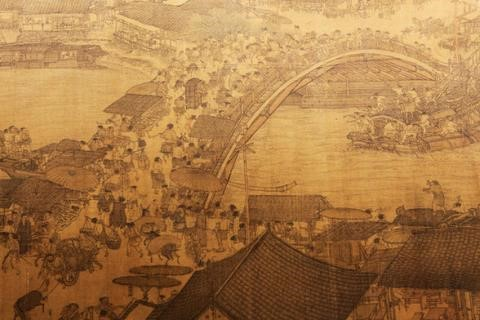
\includegraphics[width=1.1\textwidth]{images/Hinh 4a.jpg}
    \begin{center}
      \figurename{ 4a: Tác phẩm \textit{"Thanh Minh Thượng Hà Đồ"} của Trương Trạch Đoan.}
    \end{center}
  \end{minipage}
  \hfil
  \begin{minipage}{6cm}
    \centering
    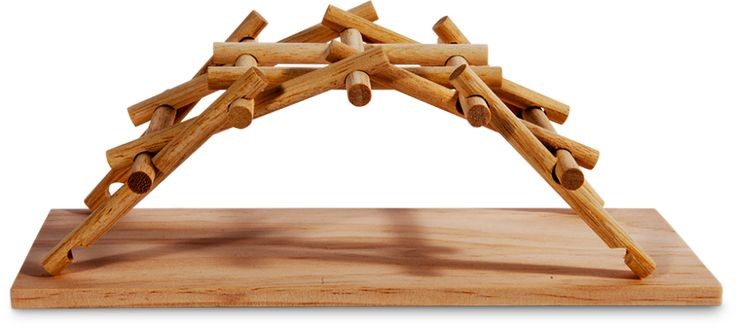
\includegraphics[width=1.3\textwidth]{images/Hinh 4b.jpg}
    \begin{center}
      \figurename{ 4b: Mô hình cầu gỗ ghép.}
    \end{center}
  \end{minipage}
\end{figure}

\begin{figure}
  \centering
  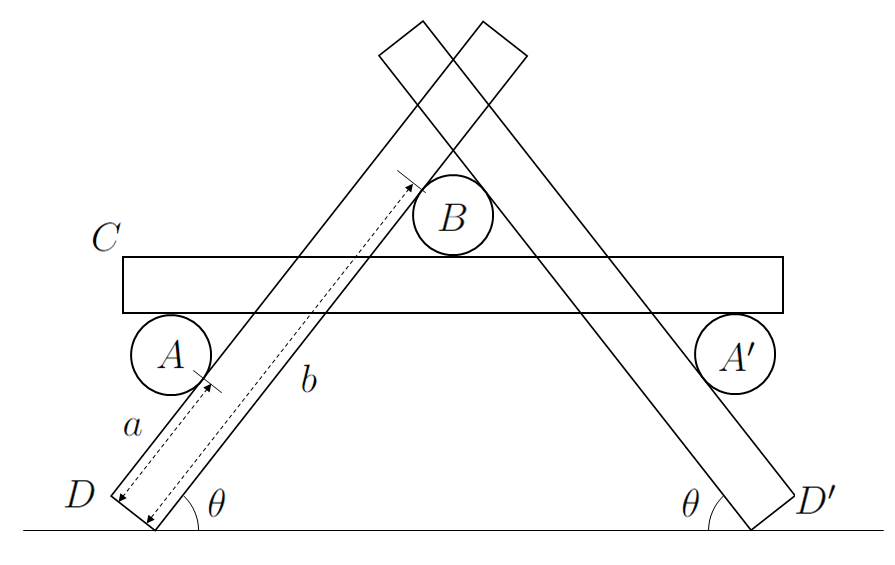
\includegraphics[width=0.55\textwidth]{images/Hinh 4c.PNG}
  \begin{center}
    \figurename{ 4c: Mô hình cầu gỗ ghép đơn giản.}
  \end{center}
\end{figure}

\begin{figure}[h]
  \centering
  \begin{minipage}{5cm}
    \centering
    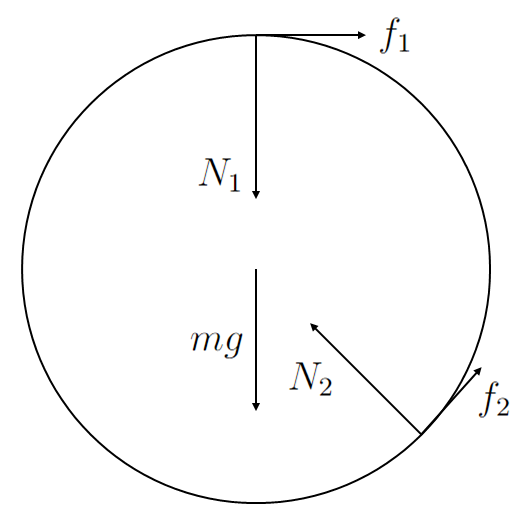
\includegraphics[width=1.1\textwidth]{images/Hinh 4d.PNG}
    \begin{center}
      \figurename{ 4d: Các lực tác dụng lên thanh A.}
    \end{center}
  \end{minipage}
  \hfil
  \begin{minipage}{5cm}
    \centering
    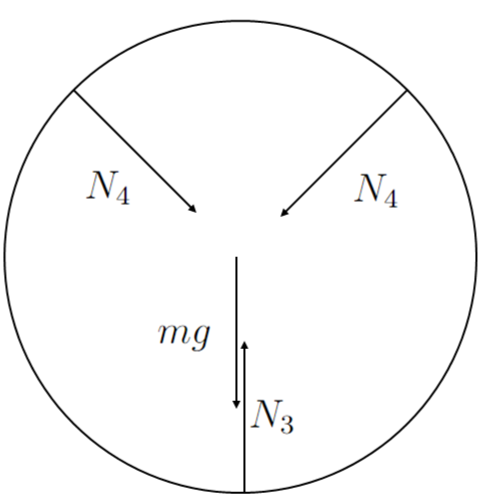
\includegraphics[width=1.08\textwidth]{images/Hinh 4e.PNG}
    \begin{center}
      \figurename{ 4e: Các lực tác dụng lên thanh B.}
    \end{center}
  \end{minipage}
\end{figure}

\indent Trên hình 4c là một mô hình cầu gỗ ghép đơn giản gồm 3 phần. Trong mô hình này, ta sẽ xem xét sự cân bằng của cầu gỗ trong mặt phẳng thẳng đứng, mỗi cặp thanh dài song song với mặt giấy được xem như một thanh có khối lượng $M$, nhờ đó cầu gỗ ghép có thể được đơn giản hoá thành 6 thanh: 3 thanh ngắn $A$, $A'$, $B$ và 3 thanh dài $C$, $D$, $D'$. Tất cả các thanh đều có bán kính tiết diện $R$ và được khắc rãnh. Khối lượng của các thanh ngắn là $m$ và tất cả các thanh đều có chiều dài $L$, các thanh dài không tiếp xúc với nhau. Bề mặt của thanh ngắn $B$ là trơn và nhẵn, hệ số ma sát nghĩ giữa các thanh còn lại là $\mu$ và hệ số ma sát nghĩ giữa thanh và mặt đất là $\mu'$. Các thanh dài $D$ và $D'$ tạo với phương ngang một góc $\alpha$. Gia tốc trọng trường có độ lớn là $g$.\\
\vspace{-20px}
\begin{enumerate}
  \item Biết rằng trong hình 4c, khoảng cách từ đầu dưới của thanh $D$ đến điểm tiếp xúc với thanh $A$ là $a$, hãy xác định khoảng cách $b$ từ đầu dưới của thanh $D$ đến điểm tiếp xúc với thanh $B$.
  \item Khi hệ đang ở trạng thái cân bằng, hình 4d và 4e biểu diễn các lực tác dụng lên các thanh $A$ và $B$. Hãy biểu diễn các lực tác dụng lên các thanh $C$ và $D$. Lập phương trình cân bằng cho từng thanh $A$, $B$, $C$ và $D$.
  \item Giả sử $M=6m$, $\theta=45^{\circ}$, $L=$\SI{30}{\centi\metre}, $a=$\SI{16}{\centi\metre}, $R=2(\sqrt{2}-1)$ \SI{ }{\centi\metre}, hãy xác định điều kiện của hệ số ma sát nghỉ $\mu$ sao cho cầu có thể cân bằng. Kết quả làm tròn đến ba chữ số có nghĩa.
\end{enumerate}